%\documentclass[8pt, handout]{beamer}
%\usepackage{pgfpages} 								%Для распечатки
%\pgfpagesuselayout{2 on 1}[a4paper,border shrink=10mm]

\documentclass[8pt]{beamer}

\usepackage[english,russian]{babel}
\usepackage[utf8]{inputenc}
\usepackage{mflogo}
\usepackage{amsmath,amsfonts,amssymb}
\usepackage{euscript}
\usepackage{graphicx}
\usepackage{xcolor}
\usepackage{transparent}



\beamertemplatenavigationsymbolsempty

\usetheme{EastLansing}
\setbeamercovered{transparent}


\title[Ряды]{Математический анализ\\ Тема 5: Ряды}
\author[Выборный Е. В.]{Выборный Евгений Викторович\\ email: evybornyi@hse.ru}
\date{Москва 2016} 


\makeatletter
\setbeamertemplate{footline}{
    \leavevmode%
    \hbox{%
    \begin{beamercolorbox}[wd=.25\paperwidth, ht=2.5ex, dp=1ex, center]{author in head/foot}%
        \usebeamerfont{author in head/foot}%
        \insertshortauthor
    \end{beamercolorbox}%
    \begin{beamercolorbox}[wd=.5\paperwidth,ht=2.5ex,dp=1ex,center]{title in head/foot}%
        \usebeamerfont{title in head/foot}\insertshorttitle
    \end{beamercolorbox}%
    \begin{beamercolorbox}[wd=.25\paperwidth,ht=2.5ex,dp=1ex,right]{date in head/foot}%
        \usebeamerfont{date in head/foot}\insertshortdate{}\hspace*{2em}
        \insertframenumber{} / \inserttotalframenumber\hspace*{2ex}
    \end{beamercolorbox}}%
    \vskip0pt%
}
\makeatother

\makeatletter
\setbeamertemplate{title page}
{
\centering
 \usebeamerfont{author}\insertauthor
 \vfill
 \begin{beamercolorbox}[rounded=true,shadow=true,sep=8pt,center]{title}
  \usebeamerfont{title}\inserttitle
 \end{beamercolorbox}
\vfill
\centering
\insertdate\par
 \vskip0.2em
}
\makeatother

\begin{document}
%\parindent=1.5em %красная строка

\begin{frame}
\titlepage
\end{frame}

\begin{frame}{Числовые ряды. Определение}
В математике и различных приложениях крайне часто возникает необходимость рассматривать суммы с бесконечным числом слагаемых. Приведем два примера.
\begin{block}{Представление числа в десятичной системе счисления}
В десятичной системе счисления любое действительное число представляется в виде бесконечной десятичной дроби
$$a = a_0,d_1d_2d_3\ldots,$$
где $d_k$ --- цифра от $0$ до $9$. Эта запись означает, что
$$a = a_0+ \frac{d_1}{10}+\frac{d_2}{10^2}+\frac{d_3}{10^3}+\cdots$$

\end{block}
  
\begin{block}{Бесконечная геометрическая прогрессия}
Очевидно, что
$$\frac12+\frac14+\frac{1}{8}+\cdots = 1.$$
\begin{center}
\includegraphics<1>[scale=0.5]{geometr-series0.pdf}
\includegraphics<2>[scale=0.5]{geometr-series1.pdf}
\includegraphics<3>[scale=0.5]{geometr-series2.pdf}
\includegraphics<4>[scale=0.5]{geometr-series3.pdf}
\includegraphics<5>[scale=0.5]{geometr-series4.pdf}
\end{center}
\end{block}
\end{frame}

\begin{frame}{Числовые ряды. Определение}
\begin{block}{Определение}
Пусть задана последовательность $a_n$. Тогда символ
\vskip-0.1em
$$\sum_{k=1}^{+\infty}a_k = a_1+a_2+\cdots+a_n+\cdots,$$
\vskip-0.1em
представляющий упорядоченную сумму бесконечного числа слагаемых, называют {\bf числовым рядом}. Величины $S_n$:
\vskip-0.1em
$$S_n = \sum_{k=1}^{n} a_k = a_1+\cdots+a_n,$$
\vskip-0.1em
называют {\bf частичными суммами} числового ряда. Если последовательность числе $S_n$ имеет предел при $n\to+\infty$, то говорят, что соответствующий числовой ряд {\bf сходится}, а число
$$S= \lim_{n\to+\infty}S_n = \lim_{n\to+\infty} \sum_{k=1}^{n} a_k$$
называют {\bf суммой числового ряда}. В этом случае пишут:
$$S = \sum_{k=1}^{+\infty}a_k.$$
\end{block}
\end{frame}

\begin{frame}{Числовые ряды. Определение}
В действительности, числовые ряды --- это другой способ говорить о числовых последовательностях. 
\vskip1em
Каждому числовому ряду соответствует последовательность частичных сумм:
$$\sum_{k=1}^{+\infty} h_k\quad \rightarrow \quad S_n = \sum_{k=1}^{n} h_k.$$
Обратно, для произвольной последовательности $a_n$ можно рассмотреть числовой ряд:
$$\sum_{k=1}^{+\infty}d_k = a_1+(a_2 - a_1)+(a_3-a_2)+\cdots,$$
где
$$d_n = a_{n} - a_{n-1},\quad n\ge 2, \qquad d_1 = a_1.$$
Частичные суммы этого ряда в точности совпадают с членами последовательности $a_n$:
$$a_n = \sum_{k=1}^{n}d_k.$$
 Следовательно, если последовательность $a_n$ сходится, то и ряд с членами $d_k$ сходится, и соответствующие пределы совпадают.
\end{frame}

\begin{frame}{Числовые ряды. Примеры}
\begin{enumerate}
\item Числовой ряд
$$\sum_{k=1}^{+\infty}1 = 1+1+1+\cdots$$
расходится к $+\infty$, поскольку частичные суммы $S_n = n\to+\infty$ при $n\to+\infty$.
\item Числовой ряд
$$\sum_{k=0}^{+\infty}(-1)^n = 1-1+1-1+\cdots$$
расходится, поскольку частичные суммы $S_n$ не имеют предела.
\item Числовой ряд
$$\sum_{k=1}^{+\infty}\frac{1}{(1+k)k} =
 \sum_{k=1}^{+\infty} \left(\frac{1}{k}-\frac{1}{k+1}\right) =1$$
сходится, поскольку частичные суммы имеют вид:
$$S_n = \sum_{k=1}^n \left(\frac{1}{k}-\frac{1}{k+1}\right) =
 \left(1-\frac{1}{2}\right)+\left(\frac12 - \frac13\right)+\cdots+ \left( \frac{1}{n} - \frac{1}{n+1}\right) = 1-\frac{1}{n+1}.$$
 \item Расходится числовой ряд
 $$\sum_{n=1}^{+\infty}\ln\left( 1 + \frac{1}{n} \right) = \sum_{n=1}^{+\infty}\ln\left( \frac{n+1}{n} \right) = 
\sum_{n=1}^{+\infty}\Big( \ln(n+1) - \ln(n) \Big) = +\infty.$$
\end{enumerate}
\end{frame}


\begin{frame}{Числовые ряды. Свойства}
\begin{block}{Остаток ряда}
Числовой ряд
$$R_k=\sum_{n=k+1}^{+\infty} a_n$$
называют $k$-ым {\bf остатком ряда} $\displaystyle \sum_{n=1}^{+\infty}a_n$. Исходный ряд и его остаток сходятся или расходятся одновременно.
\end{block}

\begin{block}{Линейность}
Если ряды $\displaystyle \sum_{n=1}^{+\infty}a_n$ и $\displaystyle \sum_{n=1}^{+\infty}b_n$ сходятся, то сходится и ряд с общим членом $A\, a_n+B\, b_n$. Справедливо равенство:
$$\sum_{k=1}^{+\infty} \left( A\, a_n+B\, b_n \right) = A\sum_{n=1}^{+\infty}a_n+B\sum_{n=1}^{+\infty}b_n.$$
\end{block}
\end{frame}

\begin{frame}{Числовые ряды. Свойства}
\begin{block}{Теорема. Необходимое условие сходимости ряда}
Если числовой ряд $\displaystyle \sum_{n=1}^{+\infty}a_n$ сходится, то $a_n\to0$ при $n\to+\infty$.
\end{block}
\vskip-0.1em
\begin{block}{Доказательство}
Сходимость ряда означает, что
$$\exists\ \lim_{n\to+\infty}S_n =  \lim_{n\to+\infty}\sum_{k=1}^n a_k=S.$$
Тогда
$$a_n = S_n - S_{n-1} \quad \Rightarrow \quad
 \lim_{n\to+\infty} a_n = \lim_{n\to+\infty} S_n - \lim_{n\to+\infty} S_{n-1} = S-S = 0.$$
\end{block}
Обратное утверждение не верно. Например, ряд $\displaystyle \sum_{n=1}^{+\infty}\frac{1}{\sqrt{n}}$ расходится, поскольку
$$S_n = \frac{1}{\sqrt{1}}+\cdots+\frac{1}{\sqrt{n}} \ge n\, \frac{1}{\sqrt{n}} = \sqrt{n}\quad \Rightarrow \quad
S_n\to+\infty.$$
\end{frame}

\begin{frame}{Числовые ряды. Знакопостоянные ряды}
Ряд называют знакопостоянным, если все $a_n \ge 0$ или $a_n\le 0$.
\begin{block}{Предложение}
Положительный числовой ряд $\displaystyle \sum_{n=1}^{+\infty}a_n$, где $a_n\ge0$, всегда имеет сумму. Сумма ряда будет конечной, если последовательность частичных сумм ряда ограничена, иначе сумма ряда будет равна $+\infty$.
\end{block}
\vskip-0.1em
\begin{block}{Доказательство}
Последовательность частичных сумм является монотонной:
$$A_{n+1} = \sum_{k=1}^{n+1} a_k = A_n+a_{n+1}\ge A_n,\quad \forall n.$$
Следовательно, по теореме Вейерштрасса существует предел последовательности $A_n$, представляющий сумму ряда.
\end{block}
\end{frame}

\begin{frame}{Числовые ряды. Теорема сравнения}
\begin{block}{Теорема. Сравнение}
Рассмотрим два положительных ряда $A=\displaystyle \sum_{n=1}^{+\infty}a_n$ и $B=\displaystyle \sum_{n=1}^{+\infty}b_n$. Пусть справедливо неравенство
$$a_n\le b_n,\quad \forall n\ge 1.$$
Тогда из сходимости ряда $B$ следует сходимость ряда $A$, а из расходимости ряда $A$ следует расходимость ряда $B$.
\vskip1em
Аналогичное утверждение справедливо при выполнении условия $a_n = O(b_n)$.
\end{block}
\begin{block}{Теорема. Асимптотическое сравнение}
Пусть $a_n\ge0$, $b_n\ge 0$ и $a_n\sim b_n$, при $n\to+\infty$. Тогда ряды $\displaystyle \sum_{n=1}^{+\infty}a_n$ и $\displaystyle \sum_{n=1}^{+\infty}b_n$ сходятся или расходятся одновременно.
\end{block}
\begin{block}{Упражнение}
Выпишите полное доказательство этих теорем.
\end{block}
\end{frame}

\begin{frame}{Числовые ряды. Признак Коши}
В качестве эталона для сравнения рядов выберем геометрическую прогрессию:
$$\sum_{n=0}^{+\infty}q^n = \frac{1}{1-q},\quad 0\le q<1.$$
\vskip-0.5em
\begin{block}{Теорема. Признак Коши}
Пусть $a_n\ge0$ и для достаточно больших $n$ справедливо неравенство:
$$\mathcal{C}_n = \sqrt[n]{a_n}\le q<1.$$
Тогда ряд $\displaystyle \sum_{n=1}^{+\infty}a_n$ сходится, а если $\mathcal{C}_n \ge 1$, то ряд расходится.
\end{block}
\begin{block}{Доказательство}
Из предположения теоремы следует, что $a_n<q^n$ для достаточно больших $n$. Из теоремы о сравнение рядов и сходимости геометрической прогрессии с знаменателем $q<1$ следует сходимость ряда с членами $a_n$.
\vskip0.8em
Если $\mathcal{C}_n\ge 1$, то и $a_n\ge 1$. Следовательно, $a_n\not\to0$ при $n\to+\infty$, то есть не выполнено необходимое условие сходимости ряда. 
\end{block}
\end{frame}

\begin{frame}{Числовые ряды. Признак Коши}
Поскольку нас интересует выполнение неравенства
$$\sqrt[n]{a_n}\le q<1$$
только для достаточно больших $n$ можно сформулировать предельный признак сравнения.
\begin{block}{Теорема. Предельный признак Коши}
Пусть существует предел
$$\lim_{n\to+\infty}\sqrt[n]{a_n} = q.$$
Тогда при $q<1$ ряд $\displaystyle \sum_{n=1}^{+\infty}a_n$ сходится, а при $q>1$ расходится. Если $q=1$, то вопрос остается открытым.
\end{block}
\begin{block}{Доказательство}
Рассмотрим случай $q<1$. Дано:
$$\forall \varepsilon>0 \ \exists N:\quad |\sqrt[n]{a_n}-q|<\varepsilon\quad \forall n>N.$$
Выбирая положительное $\varepsilon=\varepsilon_0 < 1-q$, получаем, что
$$\sqrt[n]{a_n}<q+\varepsilon_0<1.$$
Остается применить признак сходимости Коши.
\end{block}
\end{frame}

\begin{frame}{Числовые ряды. Признак Коши}
\begin{block}{Пример}
Рассмотрим ряд
$$\sum_{n=1}^{+\infty}\frac{n^{2n}}{e^{n^2}}.$$
Применим предельный признак Коши:
$$\lim_{n\to+\infty}\sqrt[n]{a_n} = \lim_{n\to+\infty}\frac{n^2}{e^{n}} = 0<1.$$
Следовательно, ряд сходится.
\end{block}
\begin{block}{Упражнение}
Аналогично рассмотрите ряд 
$\displaystyle \sum_{n=1}^{+\infty} 3^n \left(\frac{n+1}{n+2}\right)^{n^2}$.
\end{block}
\end{frame}

\begin{frame}{Числовые ряды. Признак Даламбера}
Сложность применения признака Коши связана с необходимостью вычисления корня $n$-ой степени. Существует более простой признак сходимости Даламбера.

\begin{block}{Теорема. Признак Даламбера}
Пусть $a_n>0$. Если для достаточно больших $n$ справедливо неравенство
$$\mathcal{D}_n = \frac{a_{n+1}}{a_n}\le q<1,$$
то ряд $\displaystyle \sum_{n=1}^{+\infty}a_n$ сходится, а если $\mathcal{D}_n \ge 1$, то ряд расходится.
\vskip0.8em
Если существует предел
$\displaystyle \lim_{n\to+\infty} \frac{a_{n+1}}{a_n} =\lambda,$
то ряд сходится при $\lambda<1$ и расходится при~$\lambda>1$.
\end{block}
\begin{block}{Доказательство}
Рассмотрим случай $q<1$:
$$\mathcal{D}_n\le q<1\quad \Rightarrow \quad a_{n+1}\le q\, a_{n}\le q^2 a_{n-1} \le  \ldots \le q^n a_1.$$
Следовательно, $a_{n}=O(q^n)$, и ряд с членами $a_n$ сходится по теореме сравнения, где сравнение происходит с геометрической прогрессией.
\end{block}
\end{frame}

\begin{frame}{Числовые ряды. Признак Даламбера}
Признак Даламбера особенно удобно применять, если в формуле для общего члена присутствуют факториалы.
\begin{block}{Пример}
Рассмотрим ряд $\displaystyle\ \sum_{n=0}^{+\infty}\frac{1}{n!}$.
\vskip0.8em
По признаку Даламбера
$$\frac{a_{n+1}}{a_n} = \frac{n!}{(n+1)!} = \frac{1}{1+n}\le \frac12<1\quad (n\ge1).$$
Следовательно, ряд сходится.
\vskip0.8em
Нам известно, что
$$\sum_{n=0}^{+\infty}\frac{1}{n!} = e.$$
\end{block}
\vskip-1.1em
\begin{block}{Упражнение}
Аналогично рассмотрите ряд 
$\displaystyle\ \sum_{n=1}^{+\infty} n^2 \left(\frac{2}{3}\right)^n$.
\end{block}
\end{frame}

\begin{frame}{Числовые ряды. Интегральный признак}
Рассмотрим положительный числовой ряд $\displaystyle \sum_{n=1}^{+\infty} a_n$.
\begin{block}{Теорема. Интегральный признак сходимости ряда}
Пусть 
$$a_n = f(n),$$
где $f\in C[1,+\infty)$ положительна и монотонно убывает. 

Тогда ряд $\displaystyle \sum_{n=1}^{+\infty} a_n$ и интеграл $\displaystyle \int_{1}^{+\infty} f(x)dx$ сходятся или расходятся одновременно.
\end{block}
\vskip-1.1em
\begin{block}{Доказательство}
Из положительности $f$ следует, что сходимость интеграла эквивалентна ограниченности $F(x) = \int_1^x f(t)dt$, а сходимость ряда эквивалентна ограниченности последовательности частичных сумм~$S_n = \sum_{k=1}^n a_k$.

По теореме сравнения для интеграла:
$$a_{k}\le \int_{k}^{k+1}f(x)dx\le a_{k+1}\quad \Rightarrow \quad S_n \le F(n+1) \le S_{n+1}-a_{1}$$
Из последнего неравенства следует эквивалентность ограниченности $F(x)$ и $S_n$. 
\end{block}
\end{frame}

\begin{frame}{Числовые ряды. Интегральный признак}
Теорема об интегральном признаки сходимости имеет простую геометрическую интерпретацию.
\begin{center}
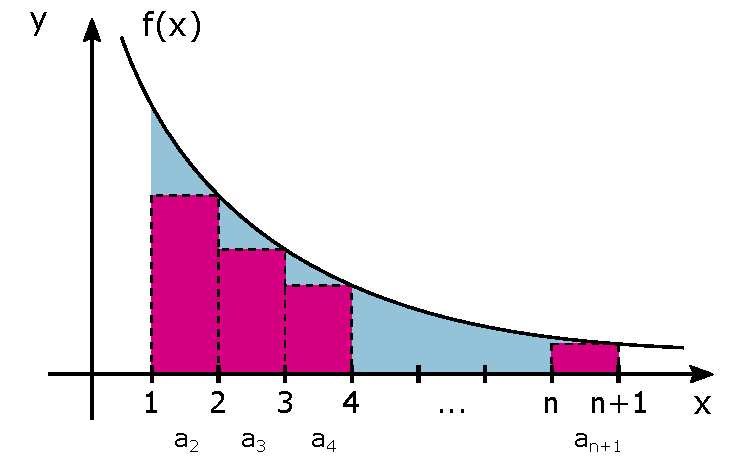
\includegraphics[scale=0.5]{thRow-Int.pdf}
\end{center}
Если интеграл $\int_1^{+\infty}f(x)dx$ сходится, то он представляет площадь под графиком $f(x)$ при $x\ge 1$. 
Сумма ряда $\displaystyle \sum_{k=2}^{+\infty}a_k$ можно интерпретировать, как площадь прямоугольников, полностью лежащих под графиком $f$. 

Следовательно, из ограниченности площади под графиком $f$ следует и ограниченность суммарной площади прямоугольников.
\end{frame}
\end{document}